\item \points{2b} {\bf Degree-k polynomial regression}


For this sub-question question, we will use the datasets provided in
the following file:
%
\begin{center}
	\texttt{src/train.csv}
\end{center}
%

This file contains two columns: $x$ and $y$. In the terminology described in the introduction, $x$ is the attribute (in this case one dimensional) and $y$ is the output label.

Using the formulation of the previous sub-question, implement linear regression with \textbf{normal equations} using the feature map of degree-k polynomials. Using the |LinearModel| provided in |src/submission.py|, this means you will be implementing the functions |fit()|, |predict()|, and |create_poly()|.  

To extend the idea above to degree-$k$ polynomials, consider $\phi:\mathbb{R}\rightarrow \mathbb{R}^{k+1}$ to be 
		\begin{align}
	\phi(x) = \left[\begin{array}{c} 1\\ x \\ x^2\\ \vdots \\x^k \end{array}\right]\in \mathbb{R}^{k+1} \label{eqn:feature-k}
	\end{align}

We will use $k=1,2,3,5,10,20$ as test cases. To verify a correct implementation, autograder test case |2b-9-basic| will create a plot in |src/large-poly.png|.  Note that test |2b-9-basic| will NOT be awarded points and is used to test if your implementation can generate a plot similar to the following:

\begin{figure}[H]
  \centering
  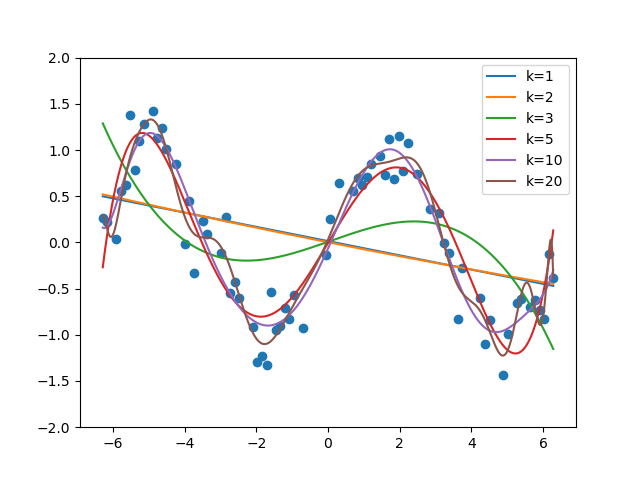
\includegraphics[width=0.65\linewidth]{02-featuremaps/large-poly.png}
  \centering
\caption{Polynomial regression with kernel sizes 1,2,3,5,10 and 20}
\end{figure}